\chapter{Outline of the project}
\label{chap:outline}

\section{Objectives}
\subsection{Primary objectives}
The goal is to build a software system, using computer vision algorithms. First of all, it should be able to estimate the frame-to-frame motion of a racing car and the momentary orientation of the camera with respect to the ground plane. Secondly, at any time, the system should be able to create a birds eye view map of the environment that is in front of the car, in particular the positions of the cones which are used to mark the drivable path.\bigskip 

\subsection{Secondary objectives}
When a good solution is found to these two problems, the system could be expanded and obstacles, side barriers etc. could be entered into the map previously mentioned. Based on the previous features of the system, two additional features could be added: reconstruction of the car's trajectory over time and building a global map from the instantaneous map.\bigskip

These last two additional features are a nice addition to the primal goals, but will only be investigated once the primal goals are working properly.\bigskip

\section{The motion model}
When we talk about motion, we have to define how this motion will be described. Equally important is to define the coordinate frames we will be working with.

\subsection{Motion parameters}
Every motion can be decomposed into three components. A motion is always happening in a certain plane, to define this plane uniquely, the normal vector $\vt$ is used. The displacement in this plane is called the translation and can be expressed by the translation vector $\vt$. The third parameter is the rotation, this can be expressed with the rotation matrix $\MR$.\bigskip

A rotation always consists of three components, a yaw, a pitch and a roll. These parameters will be discussed more thoroughly in section \autoref{ssec:rotmat}.

\subsection{Coordinate frames}
We are working with camera images, which are 2-D representations of points in a 3-D world. It is thus of utmost importance to define the coordinate frames we will be using to avoid confusion.\bigskip

First of all, there is the image itself. This is a 2-D frame with x-axis and y-axis along the horizontal axis and vertical axis of the image respectively. The unit of these coordinates is measured in pixels and the center of the frame is at the top left of the image.\textbf{ADD FIGURE}\bigskip

Secondly, there is the camera coordinate system, which we will also use for the car as the camera is rigidly attached to the car. This is a right-handed 3-D coordinate system. The center of the frame is located at the center of the camera (model). The x-axis is pointing left, the y-axis is pointing up and the z-axis is leaving the camera perpendicular to the camera in the direction of the view. \textbf{ADD FIGURE}\bigskip

The third and last coordinate frame is the real world system. This is also a right-handed 3-D coordinate system and to keep things simple, this can be defined as the camera coordinate system at frame 1.\bigskip

As we are working with three different coordinate frames, it's important to know how to transfer points from one frame to another. We'll discuss this at length in a later section.

\subsection{Motion equation}
We have talked about motion and the motion parameters. Each frame-to-frame motion will be described using these parameters in a motion equation.\bigskip

To define this equation, take two points in the real world frame: $P_1 = (X_1, Y_1, Z_1)^T$ and $P_2 = (X_2, Y_2, Z_2)^T$. The transformation from $P_1$ to $P_2$ can be described as follows:
\begin{equation}\label{eq:motion}
    \begin{pmatrix}
        X_2 \\ Y_2 \\ Z_2
    \end{pmatrix} =  \MR \begin{pmatrix}
        X_1 \\ Y_1 \\ Z_1
    \end{pmatrix}+ \vt
\end{equation}

\subsubsection{Homogeneous coordinates}
In what follows, we'll use Homogeneous coordinates instead of Cartesian coordinates. The use of Homogeneous coordinates makes some formulas easier to work with and lets us represent projective transformations by a matrix. \bigskip

To write the motion equation from \autoref{eq:motion} in Homogeneous coordinates, we take $P_1 = (X_1, Y_1, Z_1, 1)^T$ and $P_2 = (X_2, Y_2, Z_2, 1)^T$ and come to the following equation:
\begin{equation}
    \begin{pmatrix}
        X_2 \\ Y_2 \\ Z_2 \\ 1
    \end{pmatrix} = \begin{pmatrix}
        \MR & 0 \\
        0 & 0
    \end{pmatrix} \begin{pmatrix}
        X_1 \\ Y_1 \\ Z_1 \\ 1
    \end{pmatrix} + \begin{pmatrix}
        t_1 \\ t_2 \\ t_3 \\ 1
    \end{pmatrix}
\end{equation}
which can be rewritten as
\begin{equation}
    \begin{pmatrix}
        X_2 \\ Y_2 \\ Z_2 \\ 1
    \end{pmatrix} = \begin{pmatrix}
        \MR & \vt \\
        0 & 1
    \end{pmatrix} \begin{pmatrix}
        X_1 \\ Y_1 \\ Z_1 \\ 1
    \end{pmatrix}
\end{equation}
This matrix characterises the transformation or motion that occurred between two frames. Based on these transformation matrices, the position of the camera (and thus the car) can be determined by concatenating the transformations.

\subsection{Rotation matrix}\label{ssec:rotmat}
We have mentioned the rotation matrix $\MR$, but thus far it is not clear what this actually means. A rotation can always be decomposed in three components: yaw, pitch and roll. \bigskip
\begin{figure}
    \centering
    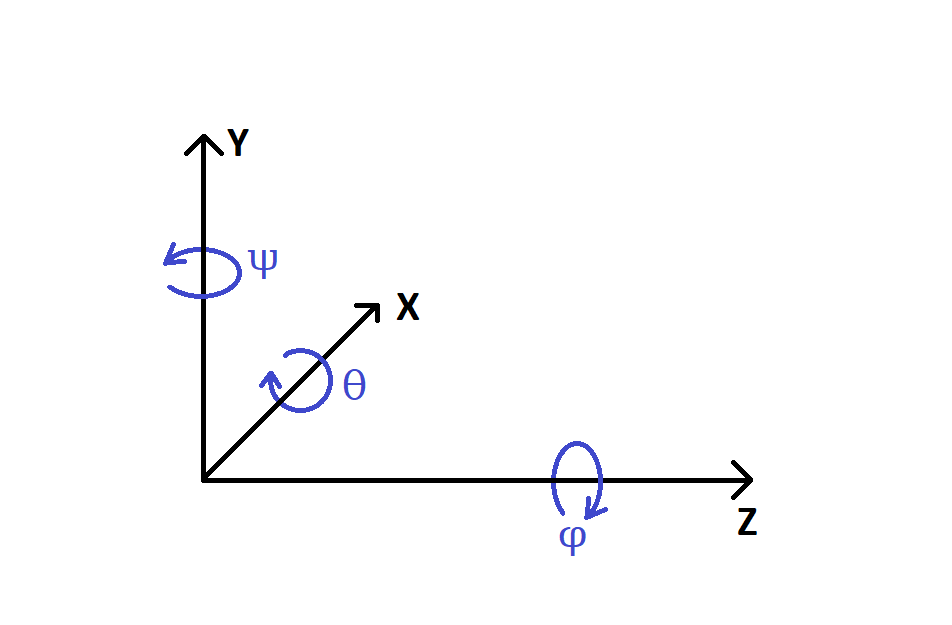
\includegraphics[width=1\textwidth]{figures/yaw_pitch_roll.png}
    \caption{Yaw, pitch and roll}
    \label{fig:rotations}
\end{figure}

\autoref{fig:rotations} shows these rotation components. $\psi$, $\theta$ and $\phi$ are yaw, pitch and roll respectively. As it is a right handed system, we have the following conventions:
\begin{itemize}
    \item When $\psi$ is positive, there is a rotation to the left.
    \item When $\theta$ is positive, there is an upward rotation.
    \item When $\phi$ is positive, there is a clockwise rotation.
\end{itemize}
This is all when looking forward from the center alongside the Z-axis.\bigskip

Each of these rotation components can be defined by a $3\times3$ matrix:
\begin{equation}
    \MR_y(\psi) = \begin{pmatrix}
        \cos\psi & 0 & \sin\psi \\
        0 & 1 & 0 \\
        -\sin\psi & 0 & \cos\psi
    \end{pmatrix}
\end{equation}
\begin{equation}
    \MR_x(\theta) = \begin{pmatrix}
        1 & 0 & 0 \\
        0 & \cos\theta & -\sin\theta \\
        0 & \sin\theta & \cos\theta \\
    \end{pmatrix}
\end{equation}
\begin{equation}
    \MR_z(\phi) = \begin{pmatrix}
        \cos\phi & -\sin\phi & 0 \\
        \sin\phi & \cos\phi & 0 \\
        0 & 0 & 1
    \end{pmatrix}
\end{equation}
To get the rotation matrix $\MR$, we multiply the yawn, pitch and roll like this:
\begin{equation}
    \MR = \MR_z(\phi)\cdot\MR_y(\psi)\cdot\MR_x(\theta)
\end{equation}
\begin{equation*}
    = \begin{pmatrix}
    \cos\psi\cos\phi & \sin\theta\sin\psi\cos\phi - \cos\theta\sin\phi & \cos\theta\sin\psi\cos\phi + \sin\theta\sin\phi \\
    \cos\psi\sin\phi & \sin\theta\sin\psi\sin\phi + \cos\theta\cos\phi & \cos\theta\sin\psi\sin\phi - \sin\theta\cos\phi \\
    -\sin\psi          & \sin\theta\cos\psi                                  & \cos\theta\cos\psi \\
  \end{pmatrix} 
\end{equation*}

\section{Determining motion}
We now have a way to describe motion in the form of a rotation matrix and a translation vector. To determine this motion, we need to have some corresponding points from each pose. Assuming we have these (we'll discuss in detail later how to get these) there are two cases, the general case where the keypoints can not all lie in one plane. However if this is the case, there's a second option to handle this.

\subsection{Essential matrix}

\subsection{Homography matrix}

\section{Visual Odometry}
To estimate the frame-to-frame motion of the racing car, footage from a camera mounted to the car is used. This process is called Visual Odometry. The changes motion induce in the images are being used to estimate that motion. Visual Odometry needs sufficient illumination in the environment, enough texture and sufficient overlap between the consecutive frames. In the following, we will break down the steps in this process.


